\section{Introduction}\label{introduction}

Rank 8 on the MMLU leaderboard, rank 17 on its STEM items. That is a real model in our sample (\texttt{Llama-3-Lumimaid-70B}), and it is not isolated: within the Top-40 aggregate pool alone, five further models disagree with their STEM standing by ten ranks or more, in both directions (\texttt{Ein-70B-v2} 21 against 41, \texttt{Qwen1.5-110B-Chat} 33 against 23). The aggregate is a single number, and the practitioner who reads it as a single ability cannot see the disagreement.

The underlying question is older than the benchmark. Whether a single ability score is psychometrically coherent has been contested since \citeauthor{spearman1904}'s (\citeyear{spearman1904}) general factor $g$: \citet{thurstone1938} showed that $g$ dissolves into separable primary abilities under factor analysis, and \citet{carroll1993} reconciled the two hierarchically, $g$ sitting above strata that remain genuinely distinct. The tension never resolved. It recurred, and it has recurred in LLM evaluation.

MMLU \citep{hendrycks2021} spans 14,042 multiple-choice items across 57 subjects and reports model accuracy as one aggregate. Is that aggregation psychometrically justified? Put more precisely: is the construct measured in College Chemistry commensurable with the one measured in Professional Law, and does their average constitute a coherent metric? Those are testable questions, and the machinery for testing them, multi-group measurement invariance, has existed in psychometrics for three decades \citep{meredith1993,vandenberg2000}. It has not been applied to a benchmark of this scale.

Our expectation of heterogeneity rests on a cognitive distinction. Episodic and semantic memory are functionally separable systems \citep{tulving1972}, and ACT-R separates declarative knowledge, the storage and retrieval of facts, from procedural knowledge, the execution of multi-step logical operations \citep{anderson1983}. We operationalize the distinction directly: Vocabulary Zipf Rarity and Named Entity Density capture a prompt's declarative retrieval demands, while the Weighted Symbolic Complexity Graph (WSCG) captures its sequential inferential load.

There is reason to expect MMLU in particular to be retrieval-weighted. \citet{wang2024} documented that performance on it has plateaued despite continued gains on reasoning-heavy benchmarks like MATH, and that Chain-of-Thought prompting fails to improve, and sometimes degrades, MMLU accuracy while yielding significant gains on their successor benchmark MMLU-Pro, concluding that MMLU is ``mostly knowledge-driven without requiring too much reasoning.'' Yet the construction of MMLU-Pro was entirely heuristic: items answered correctly by small models were removed, the distractor set was expanded from four to ten, and STEM problem sets were added. The filtering criterion operates on item difficulty ($b_{i}$) rather than discrimination ($a_{i}$), which merely restricts the measurement range by removing easy items rather than removing items that fail to differentiate models across the ability spectrum, and no psychometric criterion was specified for separating ``knowledge-driven'' from ``reasoning-driven'' items. We do not propose a new benchmark. We build and apply the measurement theory that was absent from the original one.

This is a diagnostic study, not a tool paper: the five dimensions are the instrument, and the heterogeneity they expose is the finding. We show that the mapping from structural text complexity to IRT-estimated difficulty is not invariant across MMLU's own partitions, using a joint Wald test on heteroskedasticity-consistent covariances and a permutation null that assumes nothing about the error distribution; we quantify what that costs a practitioner in displaced ranks; we trace the mechanism, a conflation of retrieval capacity with reasoning stability, to the individual model level; and we release the framework, features and IRT estimates so the audit can be repeated on any benchmark whose items are text.\footnote{The pipeline requires only free open-source resources --- Stanza (dependency parsing), SpaCy (NER), NumPyro and JAX (IRT calibration), wordfreq (Zipf frequencies), and the AMRLIB BART-AMR parser --- together with the public MMLU test set and model responses from the Hugging Face Open LLM Leaderboard.}

\section{Related Work}\label{related-work}

That aggregate benchmark scores mask construct conflation is well documented: \citet{bender2021} argue that knowledge-retrieval performance is no evidence of inferential capacity, \citet{mccoy2019} showed BERT-family models relying on surface heuristics rather than logical inference on NLI benchmarks, and high GLUE scores have been catalogued beside near-random performance on controlled reasoning probes \citep{rogers2020}. The strongest general statement is \citeauthor{bowman2021}'s (\citeyear{bowman2021}): benchmarks framed as measures of general ability rarely possess the construct validity such framing presupposes, and the field's remedy has been to build new benchmarks rather than measure the old ones \citep[see also][]{raji2021}. Those critiques are conceptual; we supply the psychometric evidence.

\citet{lalor2019} pioneered Item Response Theory for NLP benchmarks, showing that a 2PL recovers difficulty and discrimination that raw accuracy discards and that item informativeness is heterogeneous; \citet{polo2024} extended this with tinyBenchmarks, where IRT-selected subsets of roughly 100 items recover full rankings. Both assume unidimensionality, a single $\theta_{j}$ per model, and so cannot detect whether that dimension conflates separable constructs. We use the 2PL as a calibration backbone and add multi-group analysis to test the assumption.

The natural alternative is multidimensional IRT \citep{reckase2009}. We chose 2PL plus a priori stratification deliberately: MIRT's factors are recovered from the response matrix and interpreted post hoc, making the dimensions a product of the analysis rather than a hypothesis it can fail, whereas a partition fixed by MMLU's own designers can fail. It is the weaker instrument and the stronger test. Formally the procedure is a multi-group test of measurement invariance, standard since \citet{meredith1993} and reviewed by \citet{vandenberg2000}.

Predicting difficulty from text has precedent in educational measurement: \citet{embretson1987} showed that cognitive complexity features predict Rasch difficulty in reading comprehension items, at levels we return to in Section~\ref{sec:global}. In NLP, \citet{vania2021} applied IRT across 29 test sets to identify which benchmarks separate strong models, treating item parameters as the object of comparison rather than a quantity to be explained; they neither predict difficulty from text nor test invariance. Domain-targeted evaluations such as ARC \citep{clark2018} and AGIEval \citep{zhong2023} approach the problem from the other side, by isolating reasoning types; our results say such disaggregation is necessary, not merely possible.

Our syntactic indicators rest on \citeauthor{gibson1998}'s (\citeyear{gibson1998}, \citeyear{gibson2000}) Dependency Locality Theory, on which processing cost rises with the distance between dependent elements, validated in eye-tracking \citep{demberg2008} and operationalized as Mean Dependency Distance \citep{liu2008}. Because written English minimizes dependency length where it can \citep{temperley2007,gildea2015}, unusually long dependencies are a marked and costly departure; \citet{levy2008} offers a complementary expectation-based account, and our indicators capture the locality component. Table~\ref{tab:indicators} grounds the remaining dimensions.

\section{Measurement Framework and Methodology}\label{measurement-framework-and-methodology}

\subsection{Data and Response Matrix}\label{data-and-response-matrix}

We use the complete MMLU test set ($I = 14{,}042$ items across 57 subjects) and a model population of $J = 1{,}000$ open-weights language models drawn from the Hugging Face Open LLM Leaderboard \citep{beeching2023}, spanning the Deepseek, Falcon, Llama, Mistral, Pythia, Qwen, Solar, Yi, and MOE (Mixture-of-Experts) families, with parameter counts from 3.2 million to over 180 billion.

The binary response matrix $\mathbf{Y} \in \{ 0,1\}^{J \times I}$, where $Y_{ji} = 1$ if model $j$ answers item $i$ correctly, yields approximately 14 million individual response observations.

\subsection{Latent Parameter Calibration via Item Response Theory}\label{latent-parameter-calibration-via-item-response-theory}

Item difficulty parameters are estimated using the Two-Parameter Logistic model \citep{birnbaum1968,lord1968}:

\[P(Y_{ji} = 1 \mid \theta_{j},a_{i},b_{i}) = \frac{1}{1 + \exp\left( - a_{i}(\theta_{j} - b_{i}) \right)}\]

where $\theta_{j}\in\mathbb{R}$ is the latent ability of model $j$, $b_{i}\in\mathbb{R}$ the difficulty of item $i$ (the ability at which $P = 0.5$), and $a_{i} > 0$ the discrimination governing the steepness of the item characteristic curve. The standard normal prior $\theta_{j}\sim\mathcal{N}(0,1)$ resolves the location-scale indeterminacy inherent in the 2PL parameterization.

Estimation is by Stochastic Variational Inference in NumPyro and JAX rather than Joint Maximum Likelihood, which suffers from the incidental parameters problem \citep{neyman1948}: the nuisance parameters $\{\theta_{j}\}$ grow with $J$, so item estimates stay inconsistent even asymptotically. SVI marginalizes over the ability distribution and scales to the full $14{,}042 \times 1{,}000$ matrix, prohibitive under Gauss--Hermite quadrature. Priors are $b_{i}\sim\mathcal{N}(0,1)$ and $a_{i} \sim \text{HalfNormal}(1.0)$, the latter giving positivity without log-transformation;\footnote{A log-normal prior yields difficulties correlated at $r > 0.99$ with those reported here.} with 1,000 models per item the likelihood dominates the prior. Approximations are mean-field Gaussians over 5,000 iterations with Adam ($\eta = 0.01$), and we report the posterior median, since the half-normal prior on $a_{i}$ induces right-skewed posteriors (cf.\ \citealp{nunnally1994}).

Difficulty spans $b_{i} \in [-5.00, 7.12]$ ($\mu = 0.04$, $\sigma = 2.24$), discrimination $a_{i} \in [0.00, 6.07]$ ($\mu = 1.85$), and ability $\theta_{j} \in [-2.02, 3.14]$ ($\sigma = 1.03$). A Rasch refit moves the domain contrast very little (Appendix~\ref{sec:robustness}).

\subsection{Split-Sample Reliability}\label{split-sample-reliability}

Are the difficulties properties of the items or of the model sample? Splitting the 1,000 models into two cohorts ($J_{1} = J_{2} = 500$) and calibrating separately, the two difficulty vectors correlate at $r_{hh} = 0.9921$ across all 14,042 items, which Spearman--Brown converts to a full-test reliability of $0.9960$. The estimates are therefore effectively free of incidental measurement error from model sampling, and disattenuation corrections on the downstream $R^{2}$ values are unnecessary.

\subsection{A Priori Domain Grouping}\label{a-priori-domain-grouping}

The multi-group analysis requires a partition fixed before any model is estimated; grouping post hoc on response patterns or text features would introduce selection bias and inflate the test statistics. We therefore adopt the official taxonomy of MMLU's designers \citep{hendrycks2021}: $I_{\text{STEM}} = 3{,}153$ items across 19 subjects, hypothesized to require procedural inference, against $I_{\text{non-STEM}} = 10{,}889$ across 38, hypothesized to lean on declarative knowledge.

The dichotomy is imperfect --- College Biology involves substantial retrieval, Formal Logic and Jurisprudence substantial inference --- but strict adherence to the published taxonomy guarantees the test is not optimized to produce a significant result, and the partition is never modified after the fact. That mathematics and science learning recruits partly distinct processes from verbal and social reasoning is well established \citep{newcombe2009}, which supports the boundary as meaningful if coarse.

\subsection{The Five-Dimension, Nine-Indicator Framework}\label{the-five-dimension-nine-indicator-framework}

Item complexity is operationalized as five separable dimensions extracted deterministically from the prompt, because two items can share word counts and syntactic structure while differing in logical nesting, abstractness or factual obscurity. Each is grounded in an established cognitive or linguistic theory and computed without any stochastic component. Table~\ref{tab:indicators} gives definitions, grounding and distributions; three construction details do not reduce to a table entry.

\begin{table*}[t]
\centering\scriptsize
\setlength{\tabcolsep}{5pt}
\begin{tabular}{@{}>{\raggedright\arraybackslash}p{0.240\textwidth}
                  >{\raggedright\arraybackslash}p{0.485\textwidth}
                  >{\raggedright\arraybackslash}p{0.185\textwidth}@{}}
\toprule
\textbf{Indicator} & \textbf{Definition} & \textbf{Range (centre)} \\
\midrule
\multicolumn{3}{@{}l}{\emph{Dimension 1 --- topological reasoning load;} procedural knowledge in ACT-R \citep{anderson1983}} \\
\addlinespace[3.5pt]
WSCG Depth ($W_\mathrm{scg}$) & Weighted longest path $\max_{p \in \mathcal{P}}\sum_{v \in p} w(v)$ through the symbolic complexity DAG & $[0.00, 32.50]$, $\mu = 4.09$ \\
\addlinespace[4.5pt]
WSCG Nodes ($N_\mathrm{scg}$) & Operational nodes in that DAG: distinct reasoning operations or leaves & $[0, 396]$, $\mu = 20.72$ \\
\midrule
\multicolumn{3}{@{}l}{\emph{Dimension 2 --- syntactic complexity;} Dependency Locality Theory \citep{gibson1998,gibson2000}} \\
\addlinespace[3.5pt]
Syntactic MDD ($D_\mathrm{mdd}$) & $\frac{1}{n_{i}-1}\sum_{t=2}^{n_{i}}|t - h(t)|$ over the Stanza parse, $h(t)$ the head index of token $t$ \citep{liu2008} & $[0.00, 7.05]$, SD $0.64$ \\
\addlinespace[4.5pt]
Syntactic Depth ($H_\mathrm{syn}$) & Longest leaf-to-root path in the dependency tree & $[0, 19]$, SD $1.91$ \\
\midrule
\multicolumn{3}{@{}l}{\emph{Dimension 3 --- epistemological specificity;} declarative knowledge in ACT-R \citep{anderson1983}} \\
\addlinespace[3.5pt]
Entity Density ($D_\mathrm{ner}$) & $|E_\mathrm{ner}| / N_\mathrm{tokens}$, named-entity tokens from SpaCy NER & $[0\%, 100\%]$, $\mu = 6.99\%$ \\
\addlinespace[4.5pt]
Vocabulary Zipf Rarity ($R_\mathrm{zipf}$) & $\frac{1}{|V_{z}|}\sum_{w \in V_{z}}(8.0 - Z(w))$ over content words; $Z$ is the wordfreq Zipf frequency \citep{speer2022}, 8.0 maximal commonality & $[2.04, 6.86]$, $\mu = 3.52$ \\
\midrule
\multicolumn{3}{@{}l}{\emph{Dimension 4 --- semantic complexity;} syntax/semantics double dissociation \citep{berndt1996}} \\
\addlinespace[3.5pt]
Lexical Concreteness ($C_\mathrm{bry}$) & $\frac{1}{|V_{c}|}\sum_{w \in V_{c}}\mathrm{conc}(w)$ over covered words, on the \citet{brysbaert2014} 1--5 norms, higher $=$ more concrete & $[1.32, 4.80]$, $\mu = 2.36$ \\
\addlinespace[4.5pt]
AMR Depth ($D_\mathrm{amr}$) & Longest path through the BART-AMR semantic DAG \citep{banarescu2013}: conceptual nesting, surface syntax stripped & $[2, 17]$, $\mu = 6.14$ \\
\midrule
\multicolumn{3}{@{}l}{\emph{Dimension 5 --- adversarial logic structure;} non-monotonic inference under negation} \\
\addlinespace[3.5pt]
Adversarial Negation ($\widetilde{S}_\mathrm{neg}$) & OLS residual of raw negation scope on token count & $[-23.88, 55.79]$, $\mu = 0.00$ \\
\bottomrule
\end{tabular}
\caption{The five dimensions and nine complexity indicators. Every indicator is computed deterministically from the prompt text; ranges and central tendencies are over all $N = 14{,}042$ items.}
\label{tab:indicators}
\end{table*}

\textbf{Weighted Symbolic Complexity Graph.}\label{sec:d1} Consider two items of comparable length: one asks for the definition of an enzyme, the other what happens to reaction rate if temperature rises while a competitive inhibitor is present, unless the substrate is saturated. The second chains conditions the first does not, and no length- or readability-based measure separates them. Dimension 1 is built to. For each prompt we construct a node-weighted directed acyclic graph $G_{w} = (V,E,w)$: using the Stanza parse, $V$ is restricted to operational tokens drawn from a cognitive lexicon of 13 categories plus a symbolic-operator class, each vertex carrying a weight $w(v) \in [0.0, 5.0]$ on eight active tiers (the full lexicon ships with the code) matching its theoretical inferential friction (boolean conjunctions $1.0$, causative conditionals $4.0$, LaTeX integrals $5.0$). Edges come from dependency arcs, plus state-tracking edges when an entity in sentence $i$ reappears in sentence $j > i$. Since DAG path algorithms evaluate edge rather than node weights, WSCG Depth maps each target node's weight onto its incoming edge before solving the longest path.

The weights are ordinal rankings of cognitive load, not calibrated interval values, so we test whether the results depend on them: perturbing the tiers by $\pm 1.0$, uniformly, one tier at a time, and over 100 Monte Carlo draws, leaves all three primary conclusions intact in every one of 123 schemes (Appendix~\ref{sec:sensitivity}).

\textbf{Zipf rarity imputation.} Two prompts can be syntactically and logically identical while differing in obscurity: the capital of France and the capital of Kyrgyzstan are structurally equivalent, but the latter needs a fact orders of magnitude rarer in pretraining. Items with no scorable content word take the population mean for $R_{\text{zipf}}$ and so contribute no explanatory variance, a conservative limitation that bites hardest on abstract STEM items.

\textbf{Adversarial negation residualization.}\label{sec:d5} Transformers fail in known ways on truth-value inversion, and Dimension 5 targets those structures: negation operators (\emph{unless}, \emph{except}) whose scope demands non-monotonic inference. We count tokens in the dependency scope of triggers from a 59-term lexicon to obtain the raw scope $S_{\text{neg}}$. Raw scope correlates with sentence length, so part of what it measures is verbosity; the structural property is isolated by OLS residualization:

\[S_{\text{neg}} = \beta_{0} + \beta_{1}N_{\text{tokens}} + {\widetilde{S}}_{\text{neg}}\]

\noindent The residual is orthogonal to prompt length by the algebraic properties of OLS ($\text{Cov}({\widetilde{S}}_{\text{neg}},N_{\text{tokens}}) = 0$). This is equivalent to including word count as a covariate in the full path model; we residualize explicitly for interpretive transparency, and the near-unity Variance Inflation Factor reported in Section~\ref{sec:global} confirms the orthogonality held in practice.

\section{Results}\label{results}

\subsection{Global Path Analysis and Baselines}\label{sec:global}

We begin with a pooled OLS regression across all 14,042 items, regressing IRT difficulty on the nine-indicator framework as $b_{i} = \beta_{0} + \sum_{k=1}^{9}\beta_{k}X_{ki} + \epsilon_{i}$, with HC3 heteroskedasticity-consistent standard errors throughout \citep{mackinnon1985}.

\begin{table*}[t]
\centering\scriptsize
\setlength{\tabcolsep}{4pt}
\begin{tabular}{lrrrrrr}
\toprule
& \textbf{Pooled} & \multicolumn{2}{c}{\textbf{STEM}} & \multicolumn{2}{c}{\textbf{non-STEM}} & \\
\cmidrule(lr){2-2}\cmidrule(lr){3-4}\cmidrule(lr){5-6}
\textbf{Complexity Indicator} & \textbf{$b$} & \textbf{$b$} & \textbf{95\% CI} & \textbf{$b$} & \textbf{95\% CI} & \textbf{$Z$ ($p_{\text{Holm}}$)} \\
\midrule
WSCG Depth ($W_\mathrm{scg}$)                      & $0.0696^{***}$  & $0.0602$  & $[0.019, 0.102]$  & $0.0620$  & $[0.049, 0.075]$   & $-0.08$ \\
WSCG Nodes ($N_\mathrm{scg}$)                      & $-0.0023^{*}$   & $0.0189$  & $[0.006, 0.032]$  & $-0.0007$ & $[-0.003, 0.002]$  & $2.93^{\dagger}$ ($0.021$) \\
Syntactic MDD ($D_\mathrm{mdd}$)                   & $0.1654^{***}$  & $0.3694$  & $[0.217, 0.522]$  & $0.0146$  & $[-0.064, 0.094]$  & $4.05^{\dagger}$ ($3.6\times10^{-4}$) \\
Syntactic Depth ($H_\mathrm{syn}$)                 & $0.0027$        & $-0.0584$ & $[-0.129, 0.012]$ & $0.0130$  & $[-0.018, 0.044]$  & $-1.81$ \\
Zipf Rarity ($R_\mathrm{zipf}$)                    & $0.0971^{*}$    & $0.2523$  & $[0.071, 0.434]$  & $-0.0521$ & $[-0.149, 0.045]$  & $2.90^{\dagger}$ ($0.021$) \\
Entity Density ($D_\mathrm{ner}$)                  & $0.0108^{***}$  & $0.0356$  & $[0.027, 0.044]$  & $0.0002$  & $[-0.004, 0.005]$  & $7.03^{\dagger}$ ($1.8\times10^{-11}$) \\
Lexical Concreteness ($C_\mathrm{bry}$)            & $0.4127^{***}$  & $-0.1642$ & $[-0.426, 0.098]$ & $0.5883$  & $[0.444, 0.733]$   & $-4.94^{\dagger}$ ($6.4\times10^{-6}$) \\
AMR Depth ($D_\mathrm{amr}$)                       & $0.0516^{***}$  & $0.0523$  & $[-0.001, 0.106]$ & $0.0608$  & $[0.035, 0.087]$   & $-0.28$ \\
Adversarial Negation ($\widetilde{S}_\mathrm{neg}$)& $-0.0232^{***}$ & $-0.0343$ & $[-0.072, 0.004]$ & $-0.0177$ & $[-0.027, -0.008]$ & $-0.84$ \\
\bottomrule
\end{tabular}
\caption{OLS path coefficients with HC3 intervals, pooled and domain-stratified. \textbf{Pooled} ($N = 14{,}042$, intercept $-2.3975$): $R^{2} = 0.0357$, Adj.\ $R^{2} = 0.0351$, 5-fold cross-validated $R^{2} = 0.0331$, Cohen's $f^{2} = 0.0371$, residual standard error $2.20$; the HC3 Wald $F(9,14032) = 63.18$ ($p = 2.74\times10^{-114}$). \textbf{STEM} ($I = 3{,}153$): $R^{2} = 0.0792$, Adj.\ $R^{2} = 0.0766$, $R^{2}_{\mathrm{cv}} = 0.0732$, $f^{2} = 0.0860$. \textbf{non-STEM} ($I = 10{,}889$): $R^{2} = 0.0380$, Adj.\ $R^{2} = 0.0372$, $R^{2}_{\mathrm{cv}} = 0.0361$, $f^{2} = 0.0395$. Stars on pooled estimates give two-sided significance. $Z$ is the \citet{clogg1995} cross-group coefficient comparison test, with its Holm-corrected $p$-value over the family of nine in parentheses \citep{holm1979}; $^{\dagger}$ marks the five that survive at $\alpha = 0.05$. Benjamini--Hochberg control at $q = 0.05$ selects the same five. Pooled intervals are omitted for space and appear in the released results file. $^{***}p<0.001$, $^{**}p<0.01$, $^{*}p<0.05$.}
\label{tab:stratified}
\end{table*}

Eight of nine predictors reach significance and the omnibus test is extreme, yet the model explains 3.57\% of global variance. Multicollinearity does not explain that: Variance Inflation Factors run from $1.025$ (Adversarial Negation, near unity because of the residualization of Section~\ref{sec:d5}) to $2.379$ (WSCG Nodes), well below the conservative threshold of 5.0.

Admittedly, 3.57\% is small, and it deserves a direct defence. Three things make it the expected result rather than a failure. Predicting difficulty from cognitive text features yields $R^{2}$ of 0.10--0.30 on \emph{homogeneous} reading-comprehension pools \citep{embretson1987}; MMLU is not one pool but 57. The framework isolates only the \emph{structural} component of difficulty, and the remainder is content-specific: a logically shallow item can be hard because the relevant fact was rare in pretraining, which no feature computable from the prompt can see. And the pooled coefficients are dominated by the majority regime, since 77.55\% of items are non-STEM, diluting a STEM-concentrated signal to near-invisibility. That is a psychometric analogue of Simpson's Paradox, and the reason Section~\ref{domain-stratified-bifurcation} treats the stratified fit as the appropriate unit of analysis.

\begin{table}[t]
\centering\scriptsize
\setlength{\tabcolsep}{3.5pt}
\begin{tabular}{@{}lrrr@{}}
\toprule
\textbf{Predictor set} & \textbf{Global} & \textbf{STEM} & \textbf{n-STEM} \\
\midrule
Word count               & $0.0059$ & $0.0123$ & $0.0133$ \\
$+$ sentence count       & $0.0068$ & $0.0119$ & $0.0144$ \\
$+$ Flesch--Kincaid      & $0.0086$ & $0.0289$ & $0.0143$ \\
Nine indicators          & $\mathbf{0.0331}$ & $\mathbf{0.0732}$ & $\mathbf{0.0361}$ \\
Indicators $+$ surface   & $0.0383$ & $0.0844$ & $0.0360$ \\
\bottomrule
\end{tabular}
\caption{Cross-validated $R^{2}$ (mean over 5 folds) for nested predictor sets. Readability is Flesch--Kincaid grade level \citep{kincaid1975}. Adding the nine indicators to the readability baseline is significant in every partition: globally $F(9,14029) = 51.15$, $p = 6.4\times10^{-92}$; in STEM $F(9,3140) = 22.47$, $p = 2.1\times10^{-37}$; in non-STEM $F(9,10876) = 29.81$, $p = 6.3\times10^{-52}$. In-sample values and fold standard deviations are in Appendix~\ref{sec:robustness}.}
\label{tab:baselines}
\end{table}

Small relative to what, though, is the question, and Table~\ref{tab:baselines} answers it. Length predicts difficulty a little, sentence count adds essentially nothing, and readability adds a little more, chiefly in STEM. Against that baseline the framework captures $3.8\times$ the cross-validated variance globally and $2.5\times$ in STEM, significant at $p < 10^{-37}$ in every partition. Surface features are not redundant with it (adding them raises STEM $R^{2}_{\mathrm{cv}}$ from $0.073$ to $0.084$), but they are no substitute for it.

\subsection{Domain-Stratified Bifurcation}\label{domain-stratified-bifurcation}

To recover the signal suppressed by pooling, separate OLS regressions are estimated on each partition; coefficients, intervals and Holm-corrected cross-group tests appear alongside the pooled estimates in Table~\ref{tab:stratified}.

Structural complexity explains roughly twice as much difficulty variance in STEM as outside it, and not through in-sample optimism: cross-validated, $0.0732$ against $0.0361$. What changes across partitions, though, is not only how much variance is explained but what explains it. Five of nine indicators differ across groups after Holm correction, and three differ in ways that reorganize the interpretation.

\textbf{Syntactic MDD} ($D_{\text{mdd}}$) carries a strong positive coefficient in STEM ($b = 0.3694$, 95\% CI $[0.217, 0.522]$) and a near-zero one outside it ($b = 0.0146$, CI $[-0.064, 0.094]$; $Z = 4.05$, $p_{\text{Holm}} = 3.6\times10^{-4}$). DLT's prediction that long-distance dependencies increase processing cost holds for items requiring procedural computation but not for those requiring factual recall: a STEM constraint sitting in a subordinate clause several tokens from its referent is a genuine bottleneck, whereas a date in a relative clause is simply retrieved. \textbf{Entity Density} ($D_{\text{ner}}$) shows the largest divergence of any indicator ($Z = 7.03$, $p_{\text{Holm}} = 1.8\times10^{-11}$): in STEM each additional named entity acts as an operational constraint (a variable, a substance, a formula) compounding the reasoning chain ($b = 0.0356$), while in non-STEM the coefficient is indistinguishable from zero ($b = 0.0002$), entities there supplying associative context that facilitates recall rather than computational load. \textbf{Lexical Concreteness} ($C_{\text{bry}}$) reverses sign across the boundary ($Z = -4.94$, $p_{\text{Holm}} = 6.4\times10^{-6}$): abstract vocabulary makes non-STEM items easier and, perhaps surprisingly, does not make STEM items harder at all.

Four indicators do not differ across groups, and it is worth saying so plainly. WSCG Depth, Syntactic Depth, AMR Depth, and Adversarial Negation carry statistically indistinguishable coefficients in the two partitions. The bifurcation is specific, not global.

At the individual subject level the picture requires more care. Figure~\ref{fig:bifurcation} plots the 57 per-subject adjusted $R^{2}$ values by domain: the STEM row sits visibly to the right, but the two distributions overlap heavily. The ordering runs from High School Macroeconomics ($0.1750$), High School Computer Science ($0.1698$), Professional Accounting ($0.1670$) and College Chemistry ($0.1565$) at the top down to High School Physics ($-0.0352$), High School Biology ($-0.0211$) and Professional Law ($-0.0017$) at the bottom. Suggestive is as far as that ordering goes.

\begin{figure}[t]
\centering
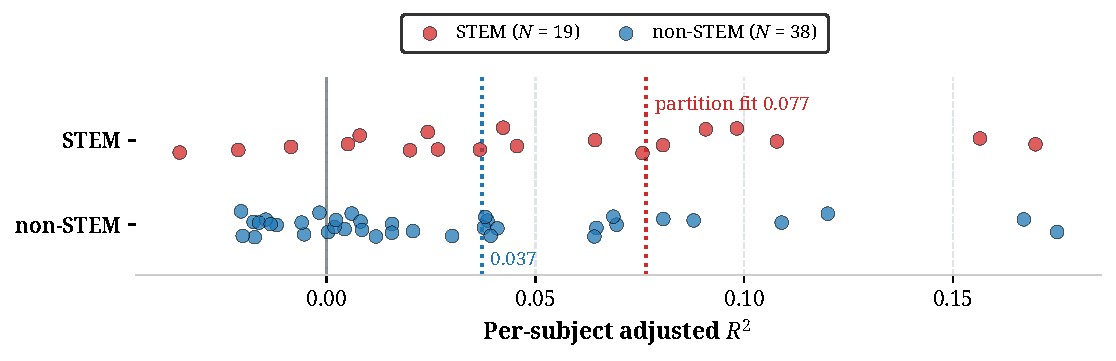
\includegraphics[width=\columnwidth]{figures/fig1_bifurcation.pdf}
\caption{Per-subject adjusted $R^{2}$, one point per subject, jittered within domain; dotted lines are the partition-level fits. The STEM distribution shifts right, but overlaps substantially.}
\label{fig:bifurcation}
\end{figure} Nine predictors against a 100-item subject pool is an 11:1 observation-to-parameter ratio, and the resulting estimates are optimistic by an amount that dwarfs the differences between them: across the 57 subjects, in-sample $R^{2}$ exceeds the repeated-cross-validation estimate by $0.232$ on average, and only three subjects retain a positive cross-validated $R^{2}$ at all (Appendix~\ref{sec:robustness}). We therefore report per-subject fit as descriptive and decline to interpret individual rankings. Treating each subject as one observation, mean adjusted $R^{2}$ is higher in STEM than outside it ($0.0520$ against $0.0311$, Cohen's $d = 0.40$) but not significantly so, $t(55) = 1.37$, $p = 0.18$. The domain effect is an item-level effect; at the subject level, with 57 noisy observations, it is underpowered.

That reassessment costs a headline and is worth the trade. A Cohen's $q$ computed from two individual subjects, College Chemistry against Professional Law, would be $0.4618$, medium-to-large but built almost entirely on overfitting. Computed where the estimates are stable, at partition level, $q = 0.0918$, bootstrap 95\% CI $[0.052, 0.136]$: small by \citeauthor{cohen1988}'s (\citeyear{cohen1988}) conventions. The honest claim is not that the domains differ enormously in how much variance structure explains, but that they differ reliably and differ in \emph{which} structure explains it, which is what Section~\ref{sec:invariance} tests.

Two outliers cut against the taxonomy and are stable enough to mention. Business Ethics and High School Macroeconomics, both non-STEM, show high structural sensitivity, consistent with multi-step conditional reasoning rather than recall; Macroeconomics is one of the three subjects whose fit survives cross-validation ($R^{2}_{\mathrm{cv}} = 0.130$), so it is not an artefact. Conversely High School Physics and Biology show negative adjusted fit, likely reflecting more straightforward recall items than their STEM label implies.

\subsection{Testing Invariance}\label{sec:invariance}

The coefficient differences in Table~\ref{tab:stratified} are descriptive. Do they constitute a statistically significant violation of structural homogeneity? Four tests answer the question, deliberately resting on different assumptions.

The primary test is a joint Wald test of coefficient equality. Let $\boldsymbol{\delta} = \widehat{\boldsymbol{\beta}}_{\text{STEM}} - \widehat{\boldsymbol{\beta}}_{\text{non-STEM}}$ be the nine-vector of slope differences. The partitions are disjoint, so their sampling errors are independent and the covariance of the difference is the sum of the two HC3 covariance matrices:

\[W = \boldsymbol{\delta}^{\top}\left(\widehat{\mathbf{V}}^{\text{HC3}}_{\text{STEM}} + \widehat{\mathbf{V}}^{\text{HC3}}_{\text{non-STEM}}\right)^{-1}\boldsymbol{\delta} \ \sim\ \chi^{2}_{9}\]

\noindent This yields $W = 138.36$ on 9 degrees of freedom, $p = 2.3\times10^{-25}$. Including the intercept raises it to $W(10) = 375.76$, but that comparison is less interesting: STEM items are simply harder on average ($\bar{b} = 0.589$ against $-0.115$), and an intercept shift is a difference in level, not in the mapping. The slopes-only test is the one that speaks to invariance.

Why not report only the likelihood ratio test, as the multi-group SEM literature would \citep{kline2016}? Because it would be inconsistent with the rest of our inference. The nested LRT compares the pooled model against the freely-estimated pair, $\Lambda = 2(\ln L_{H_{1}} - \ln L_{H_{0}})$ with $\ln L_{H_{0}} = -30996.33$ and $\ln L_{H_{1}} = -30768.90$, giving $\Lambda = 454.86$ on $\Delta\mathit{df} = 11$ and $p = 1.33\times10^{-90}$ \citep{wilks1938}. That is an emphatic rejection. But those log-likelihoods are normal-theory quantities, and Appendix~\ref{sec:robustness} shows the residuals are neither normal nor homoskedastic (pooled skew $1.37$, Breusch--Pagan $130.70$, $p = 8.5\times10^{-24}$). Using robust standard errors for coefficient inference while relying on a normal likelihood for the omnibus test would rest the two halves of the argument on contradictory assumptions. We report $\Lambda$ for comparability with the invariance literature and lean on $W$.

The permutation test assumes nothing at all. Randomly reassigning the STEM label to 3,153 of the 14,042 items and refitting, 10,000 times, produces a null distribution of the between-partition $R^{2}$ gap centred near zero (mean $0.0020$, SD $0.0072$) whose largest absolute draw is $0.0315$. The observed gap is $0.0412$. Not one permutation of ten thousand reached it, and the same holds for $\Lambda$, whose null never exceeded $48.63$ against an observed $454.86$. A stratified bootstrap over items agrees: across 1,000 resamples the 95\% interval is $[374.95, 565.35]$ for $\Lambda$ and $[0.0223, 0.0651]$ for the gap, excluding zero in 1,000 of 1,000. Whatever one believes about the error distribution, the partition is doing real work.

Structural homogeneity is rejected. The relationship between text-level complexity and IRT-estimated difficulty is not invariant across MMLU's STEM and non-STEM partitions, which is the psychometric definition of measurement non-equivalence \citep{meredith1993}. Appendix~\ref{sec:robustness} adds two further checks that a sceptical reader will want: the conclusion survives refitting difficulty under a Rasch model, and it replicates in 40 of 40 random half-samples of the item pool.

\section{Consequences for Leaderboard Validity}\label{consequences-for-leaderboard-validity}

If the mapping differs structurally across domains, reading the aggregate as a unified ability measure is undermined. With 77.55\% of items non-STEM, the aggregate is already weighted toward non-STEM performance; the non-invariance of Section~\ref{sec:invariance} is what makes that weighting a measurement asymmetry rather than a counting artifact. Two consequences follow.

\subsection{Reasoning Stability Inversion}\label{reasoning-stability-inversion}

A Reasoning Sensitivity Coefficient ($\beta_{sj}$) is estimated per model: a logistic regression of binary accuracy on WSCG Depth over the STEM partition, in log-odds space to accommodate the 25\% guessing floor:

\[\ln\left( \frac{P(Y_{ij} = 1)}{1 - P(Y_{ij} = 1)} \right) = \alpha_{j} + \beta_{sj}W_{\text{scg}}\]

where the slope $\beta_{sj}$ measures how rapidly a model's log-odds of success degrade as reasoning depth increases: near zero is robustness, steeply negative is fragility.

\subsubsection{Floor-Effect Control}\label{sec:floor}

The obvious confound has to be removed first. Models near the 25\% guessing baseline cannot degrade measurably whatever the item complexity: their slopes are flat by mathematical constraint, not robustness. Low $\theta_{j}$ and floor-constraint coincide almost perfectly, so any full-sample correlation is partly an artefact of that constraint lifting. Systematic trimming quantifies it. Excluding the bottom quartile of models by estimated ability ($\theta_{j} < -0.652$, removing $n = 250$ floor-constrained models) gives $r(\theta_{j},\beta_{sj}) = -0.512$ ($p = 2.29\times10^{-51}$, $N = 750$); removing the bottom half of the ability distribution (retaining $\theta_{j} \geq -0.072$, $N = 500$) gives $r = -0.397$ ($p = 2.79\times10^{-20}$). We take the trimmed range, $r \approx -0.40$ to $-0.51$, as the estimate of the effect. The uncorrected full-sample value is $r = -0.772$ ($p = 1.27\times10^{-198}$) and should be read as an upper bound inflated by the floor, not as the finding. Figure~\ref{fig:inversion} shows both scatters side by side.

A moderate inverse relationship that survives floor correction is the more interesting result in any case: among models that can degrade, the stronger ones degrade faster, which is not what one would predict if aggregate ability and reasoning stability were the same construct. Two qualifications constrain it. $\theta_{j}$ and $\beta_{sj}$ come from overlapping subsets of the same response matrix, introducing dependency between the estimates; and the inversion is observed in STEM only.

\begin{figure*}[t]
\centering
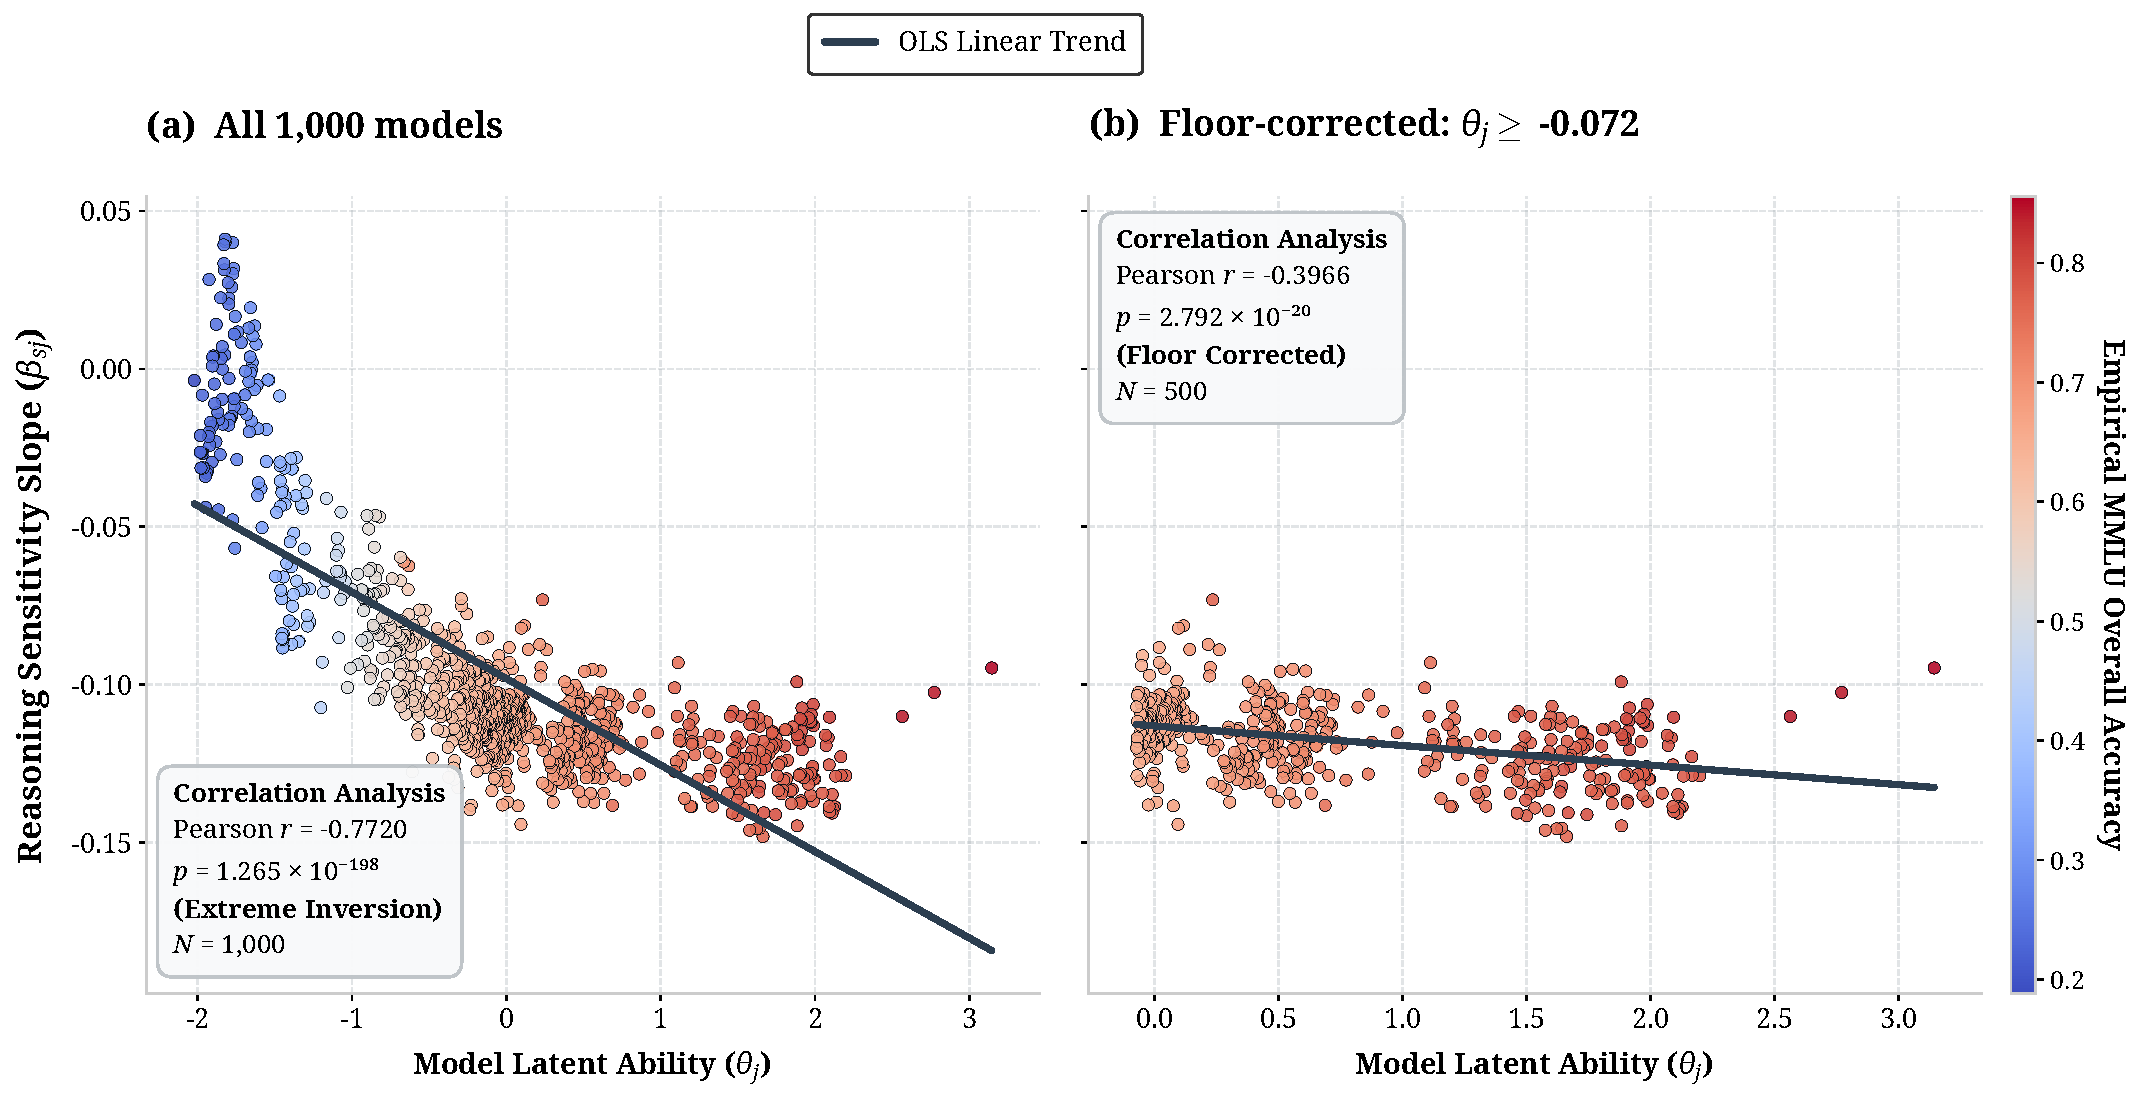
\includegraphics[width=\textwidth]{figures/fig2_inversion.pdf}
\caption{Reasoning sensitivity slopes ($\beta_{sj}$) against latent ability ($\theta_{j}$). \textbf{(a)} all 1,000 models, $r = -0.772$. \textbf{(b)} the upper half of the ability distribution, where the guessing floor no longer constrains the slope, $r = -0.397$. Both panels share a vertical scale. Point colour encodes empirical MMLU accuracy. Panel (a) is an upper bound; panel (b) is the estimate we report.}
\label{fig:inversion}
\end{figure*}

\subsection{Consequences for Downstream Model Selection}\label{consequences-for-downstream-model-selection}

In construct-validity terms \citep{cronbach1955,messick1989}, the aggregate conflates a Retrieval Capacity component with a Reasoning Stability component and weights the former more heavily. Whether that matters is an empirical question about rank stability. Weighted Kendall's $\tau$ \citep{shieh1998,vigna2015}, which penalizes displacements at the top of the leaderboard while discounting noise below, is higher against the non-STEM partition ($\tau_{w} = 0.9887$) than the STEM one ($0.9634$).\footnote{A Steiger dependent-correlation test on the underlying accuracies confirms the asymmetry formally ($Z = 208.26$), but the magnitude of that statistic reflects $J = 1{,}000$ models amplifying a small and structurally consistent difference (shared variance of $99.8\%$ against $96.8\%$) rather than a large effect. The displacement rates below are the more informative summary.}

The consequence concentrates at the frontier, where model selection happens. Of the Top 10 aggregate models, 100\% remain in the Top 10 on non-STEM items but only 80\% on STEM; of the Top 50, 92\% against 78\%. Choosing a Top-50 model on the aggregate for a STEM-focused application therefore carries a 22\% displacement rate, 11 of the 50 not in fact ranking in the top STEM tier. Ranks follow Classical Test Theory, as the public leaderboard does.

Severe displacements concentrate mid-leaderboard while the peak stays stable, because abilities are spaced non-uniformly: aggregate accuracy falls 6.22 points across the first five models but only 1.85 across Ranks 15--40, where adjacent gaps reach 0.01\%, and those 26 compressed models accumulate 246 ranks of downward STEM displacement. Stability at the top reflects population sparsity at the extreme, not a unified latent construct.

\section{Discussion}\label{discussion-1}

\subsection{Implications for Benchmark Design}\label{implications-for-benchmark-design}

The heuristic reforms of MMLU-Pro \citep{wang2024} are practically useful but theoretically insufficient. Filtering items on difficulty ($b_{i}$) removes easy items without examining why they were easy, and even filtering on discrimination ($a_{i}$) would only drop uninformative items, leaving the non-invariance of the complexity-to-difficulty mapping untouched.

Our framework supplies the missing audit. Being deterministic, it avoids the stochastic variance and API-dependence of LLM-as-annotator item classification \citep{gilardi2023}, letting researchers pre-screen item pools to check that structural reasoning load is balanced across partitions. We propose that future benchmarks report a retrieval and a reasoning index alongside any aggregate; ours is one instantiation, and the boundary between the two constructs remains open. The point applies downstream too: where reasoning stability is critical, a high aggregate score may reflect the dominant retrieval-heavy items while the model degrades on multi-step chains, so disaggregated reporting gives practitioners a better basis for deployment.

\subsection{Limitations}\label{limitations}

The framework explains a modest share of difficulty variance, and no amount of reframing changes that. What we have shown is that the share differs reliably across domains and that the pattern of predictors differs qualitatively; what we have not shown is that structural complexity is the dominant determinant of item difficulty. It is not.

Per-subject estimates deserve a second caution. With nine predictors and pools as small as 100 items, individual subject $R^{2}$ values are unreliable, cross-validated fit is negative for 54 of 57 subjects, and the subject-level contrast does not reach significance at roughly 30\% power. Only the item-level analysis, which detects $f^{2} = 0.005$ in STEM against an observed $0.086$, is adequately powered. A finer taxonomy would need larger per-cell item counts, not merely a better label set.

The WSCG weights are theoretically motivated assignments rather than calibrated interval-scale values, and although $\pm 1.0$ perturbations do not alter the primary conclusions (Appendix~\ref{sec:sensitivity}), they are not validated against human difficulty judgments. Their influence concentrates in the lowest active tier, so alternative schemes could shift the contribution attributed to reasoning load without overturning the bifurcation.

Three further boundaries. The STEM/non-STEM split is coarse, and a finer grouping would require a principled a priori taxonomy to avoid fitting the observed results. The framework sees only text, so items with images, code, diagrams or tables may carry difficulty our indicators cannot capture. And the evaluation is bounded to open-weights models; whether the fragility documented here extends to closed frontier models, whose alignment and tuning are undisclosed, remains an open and practically important question.

\subsection{Future Work}\label{future-work}

Applying the framework to successor benchmarks (MMLU-Pro, GPQA, ARC-Challenge, GSM8K) would test whether their construction resolves the heterogeneity documented here or merely displaces it to higher difficulty. Replacing our stratification with a multidimensional IRT model \citep{reckase2009} would estimate retrieval and reasoning traits without an imposed taxonomy, the natural next step now that a fixed partition has established they are separable at all. Calibrating the WSCG weights against human difficulty judgments would ground the scheme behaviourally, and extending the audit to proprietary models would show whether alignment mitigates or worsens the fragility seen here.

\section{Conclusion}\label{conclusion}

IRT calibration, multi-group path analysis and invariance testing over roughly 14 million responses from 1,000 open-weights models give a consistent answer to the question in our title. The mapping from structural text complexity to item difficulty is not invariant across MMLU's own partitions: a Wald test on heteroskedasticity-consistent covariances rejects equality at $W(9) = 138.36$, $p = 2.3\times10^{-25}$, no draw of a 10,000-fold permutation null approaches the observed divergence, and the result replicates in 40 of 40 random half-samples. Structural complexity accounts for about twice as much cross-validated difficulty variance in STEM as elsewhere, and $2.5$ to $3.8$ times as much as a readability baseline.

The cost of ignoring this is measurable. Aggregate rank tracks non-STEM accuracy more closely than STEM accuracy ($\tau_{w} = 0.9887$ against $0.9634$), so Top-50 selection displaces 22\% of the STEM-appropriate choices, and among models unconstrained by the guessing floor higher ability goes with steeper degradation under reasoning depth ($r = -0.40$ to $-0.51$). The aggregate carries systematically more information about retrieval capacity than about reasoning stability. Before we can build better evaluations, we have to know what the current ones are actually measuring.
